\documentclass{article}
\usepackage{blindtext}
\usepackage{booktabs}
\usepackage[margin=0.25in]{geometry}
\usepackage{subcaption}
\usepackage{graphicx}
\usepackage{caption}
\usepackage{hyperref}
\usepackage{pdflscape}
\usepackage{tikz}
\usepackage{threeparttable}
\usepackage{algorithmic}
\usepackage{tabularx}
\usepackage{amsmath}

\title{New Exhibits for AEJ Revisions}

\begin{document}
\maketitle
\tableofcontents
{\footnotesize 
\listoffigures
\listoftables}
\clearpage

\section{TWFE Plots}

These figures are the $\beta_\tau$'s from the TWFE regression
\begin{align}
	y_{it} = \sum_{\tau = 1910}^{2010} \beta_\tau \text{Above Med GM}_{i} \times 1\{t = \tau\} + \gamma_i + \delta_t + \epsilon_{it}
\end{align}
Where $\delta_t$ and $\gamma_i$ are decade and CZ fixed effects. Sometimes controls are included.

\clearpage
\begin{figure}
	\centering
	 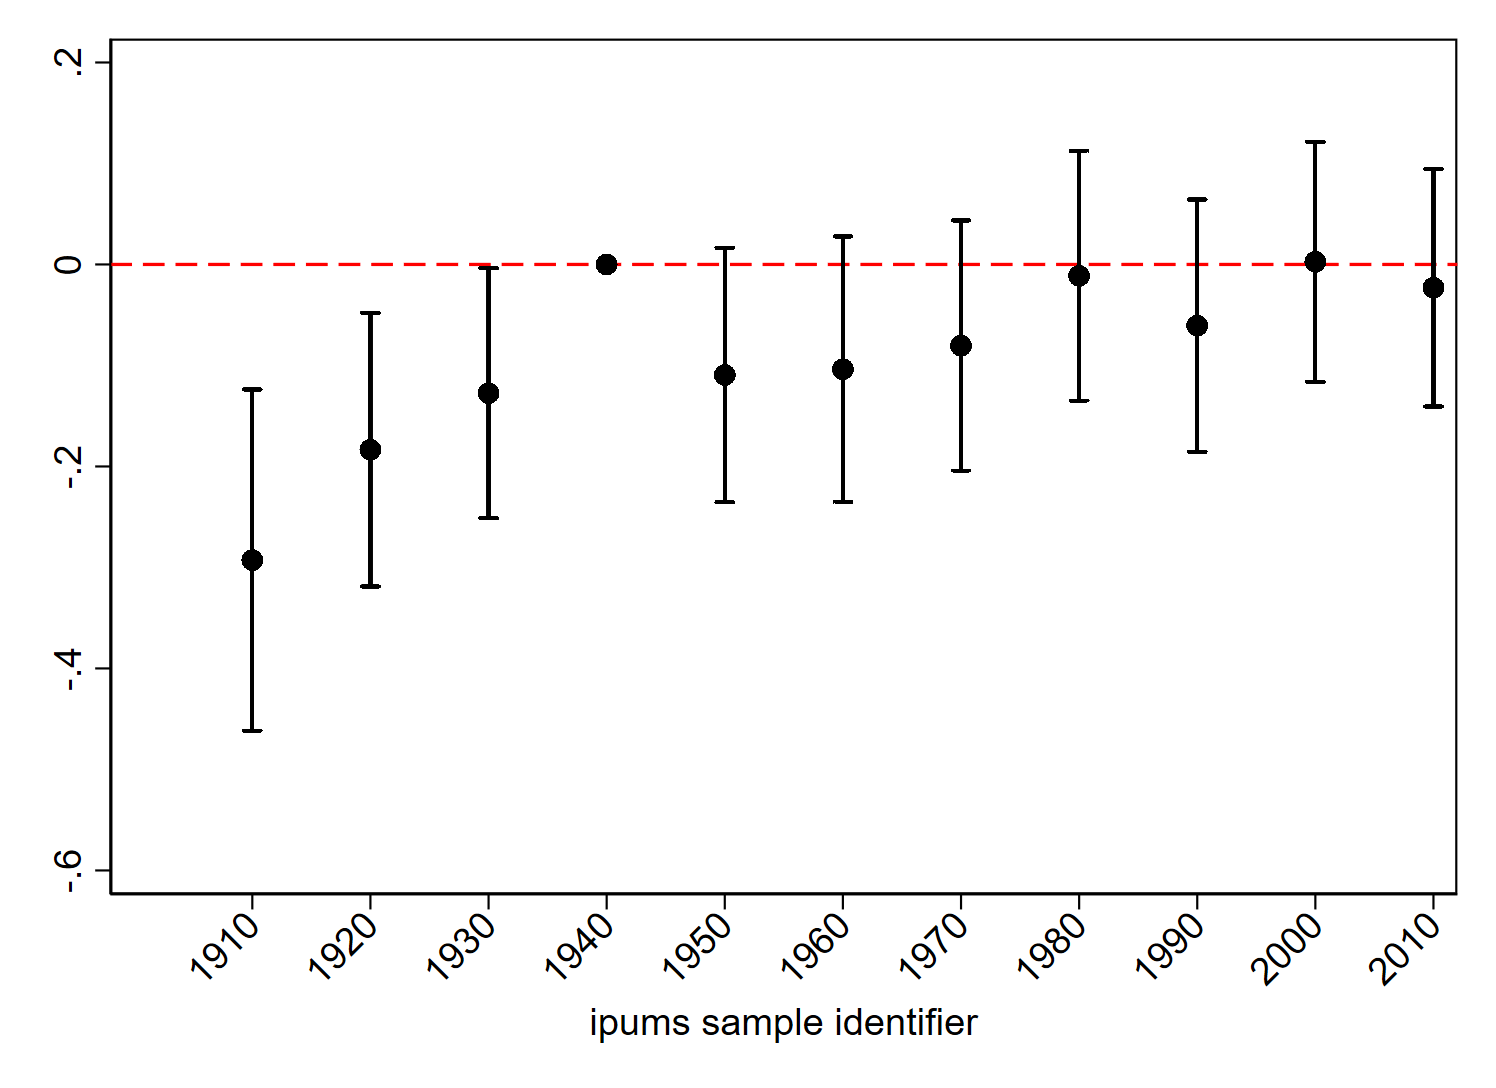
\includegraphics[width=0.7\linewidth]{figures/RR2/twfe_main.png}
	\caption{TWFE, No controls}

\end{figure}
\clearpage
\begin{figure}
	\centering
	 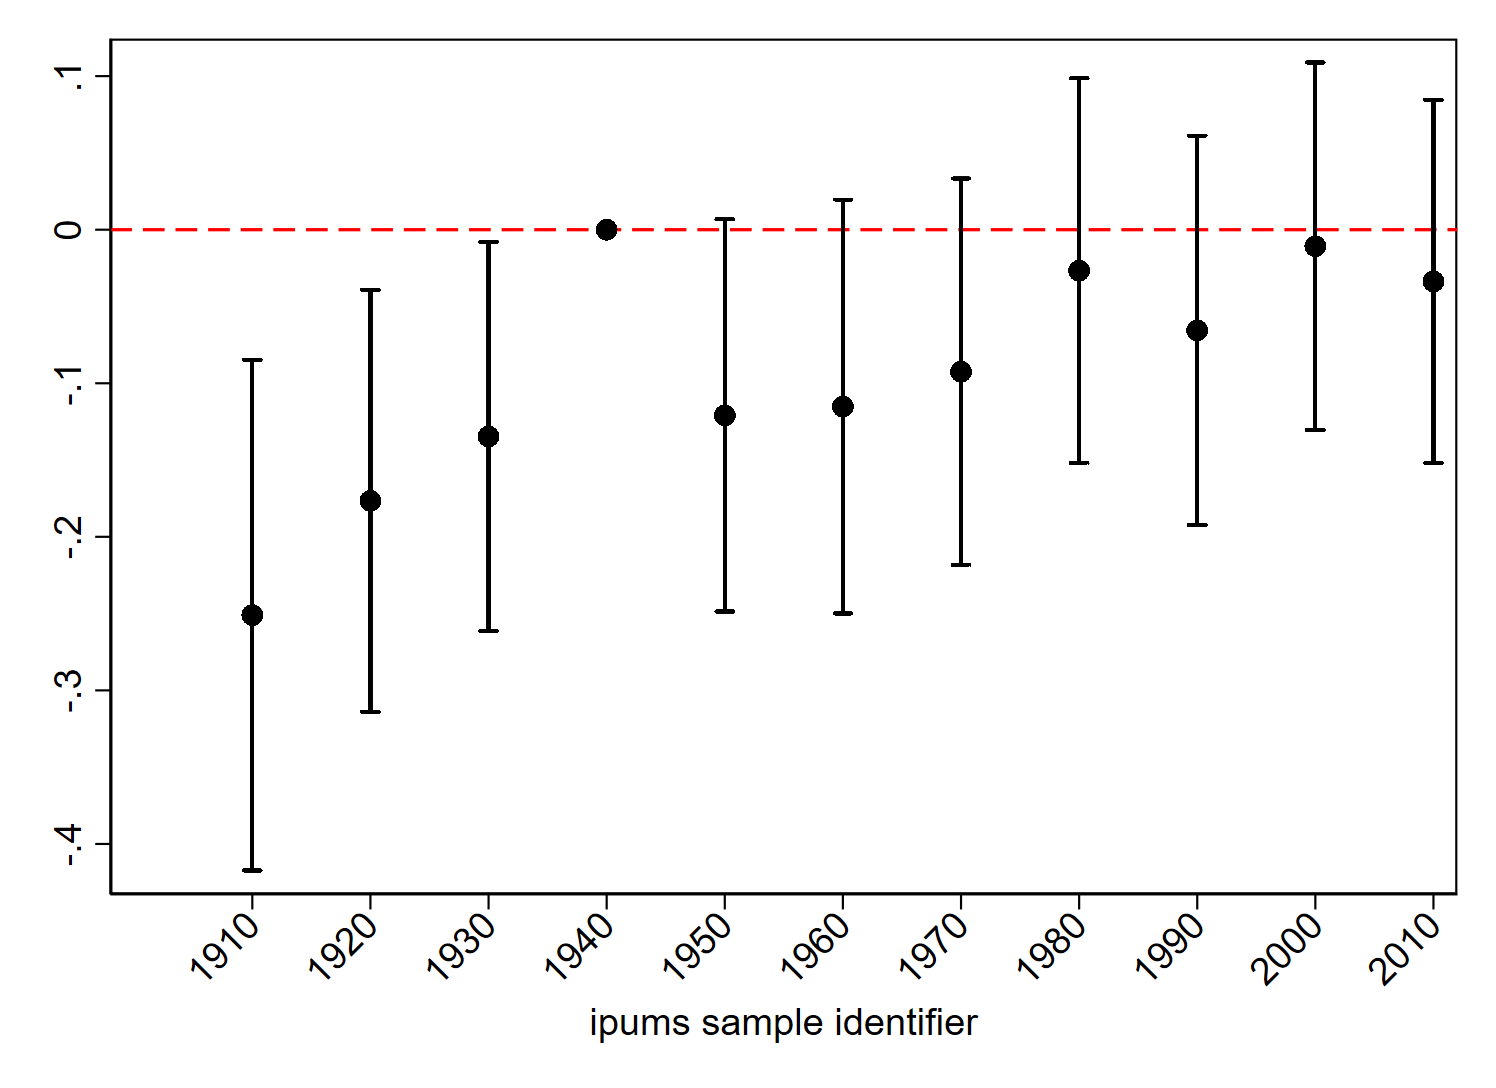
\includegraphics[width=0.7\linewidth]{figures/RR2/twfe_sumshare_base.png}
	\caption{TWFE, year X sum of shares controls}
\end{figure}
\clearpage
\begin{figure}
	\centering
	 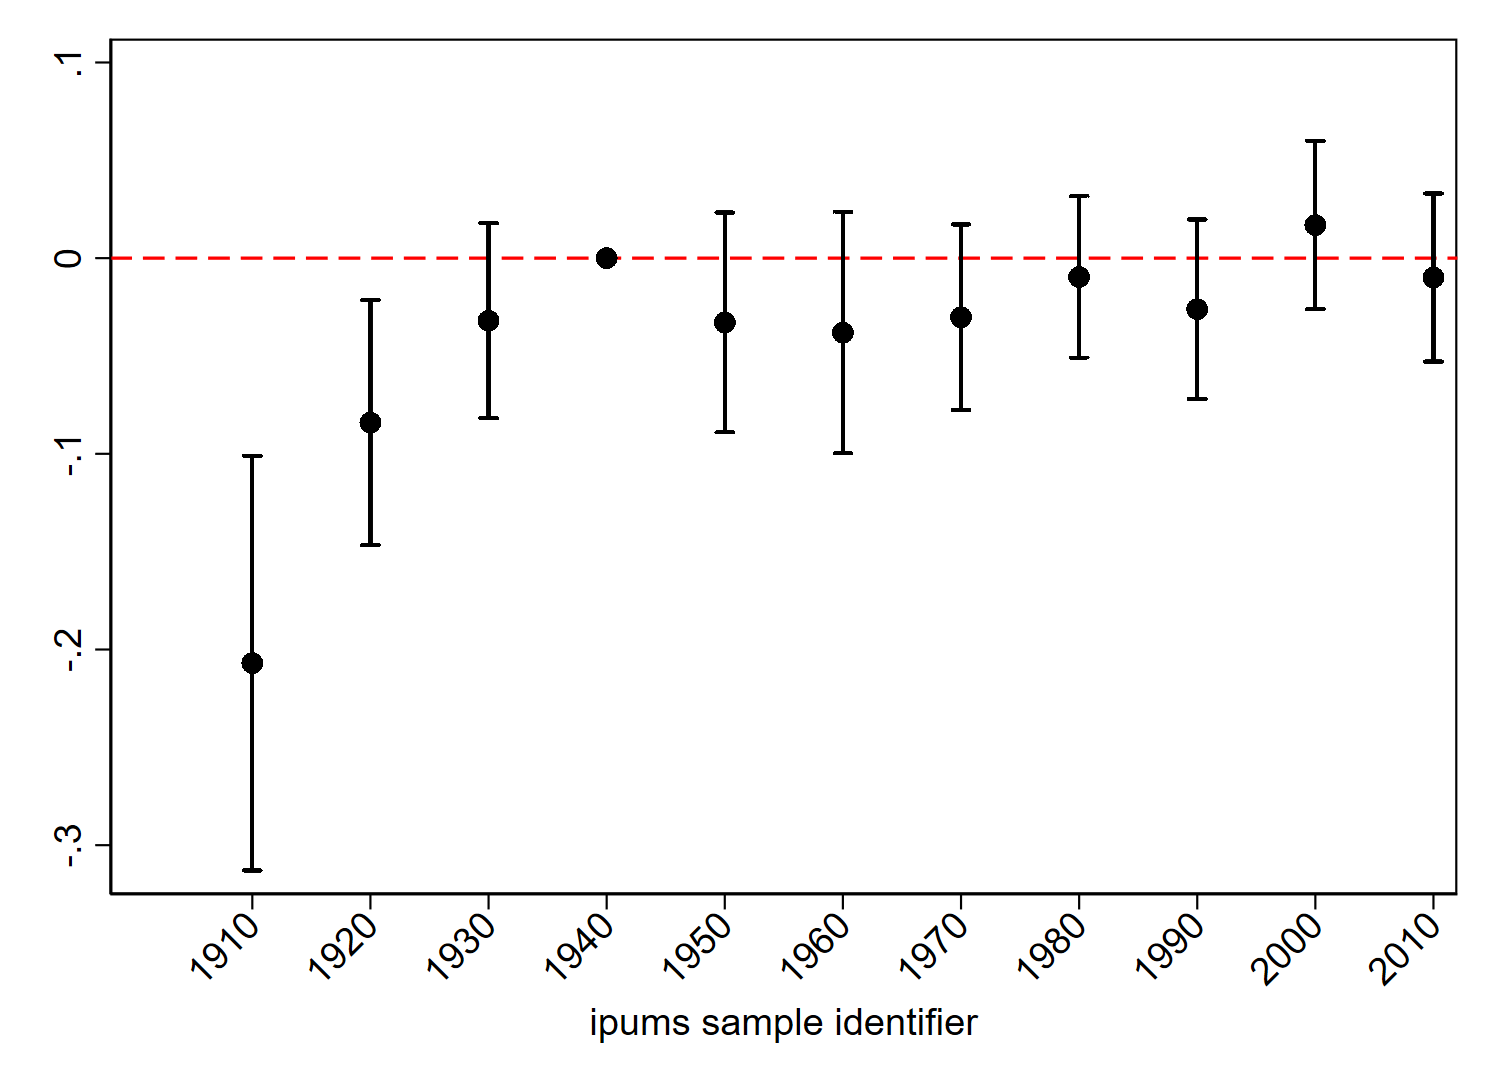
\includegraphics[width=0.7\linewidth]{figures/RR2/twfe_popgrowth.png}
	\caption{TWFE, year X population growth controls}
\end{figure}
\clearpage
\begin{figure}
	\centering
	 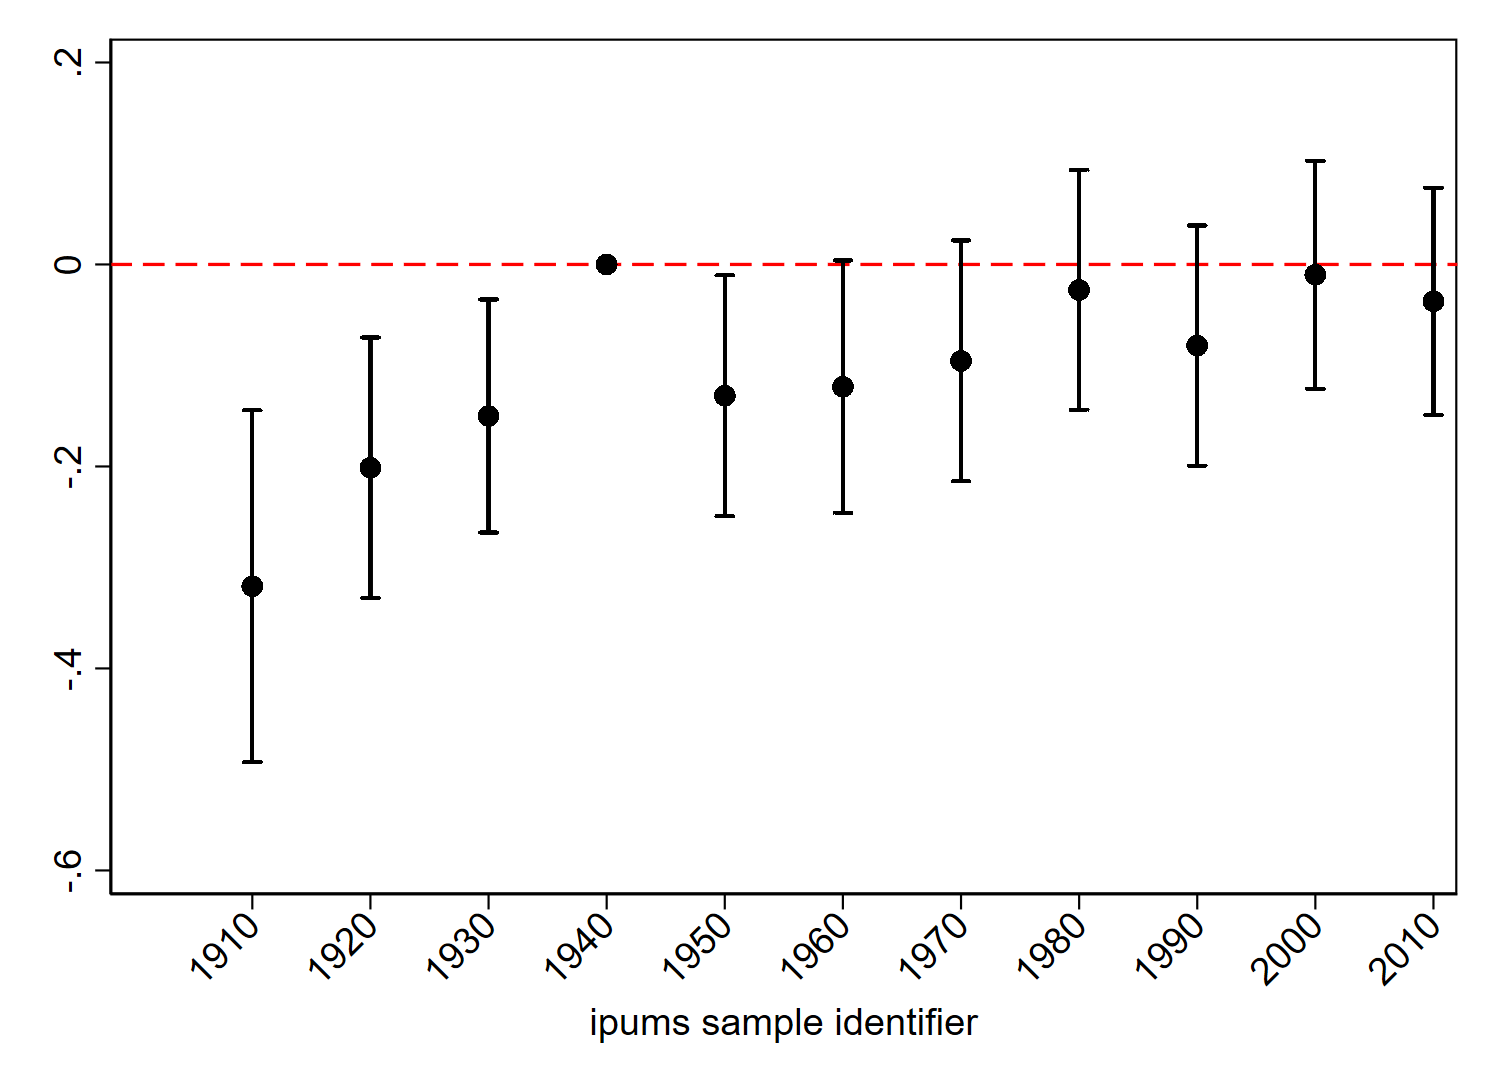
\includegraphics[width=0.7\linewidth]{figures/RR2/twfe_regions.png}
	\caption{TWFE, year X census region FEs}
\end{figure}

\clearpage
\section{Repeated Cross Section Plots}

These figures are the $\beta_t$'s from running the 2SLS regression of $t-10$ to $t$ changes $y_{it}$ on 1940-70 GM. 
\begin{align}
	y_{it} = \alpha_i + \beta_t GM_i + \mathbf{X}_i' \zeta_t + \epsilon_{it}
\end{align}
Where $X_i$ are the covariates in our main specification.


\clearpage
\begin{figure}
	\centering
	 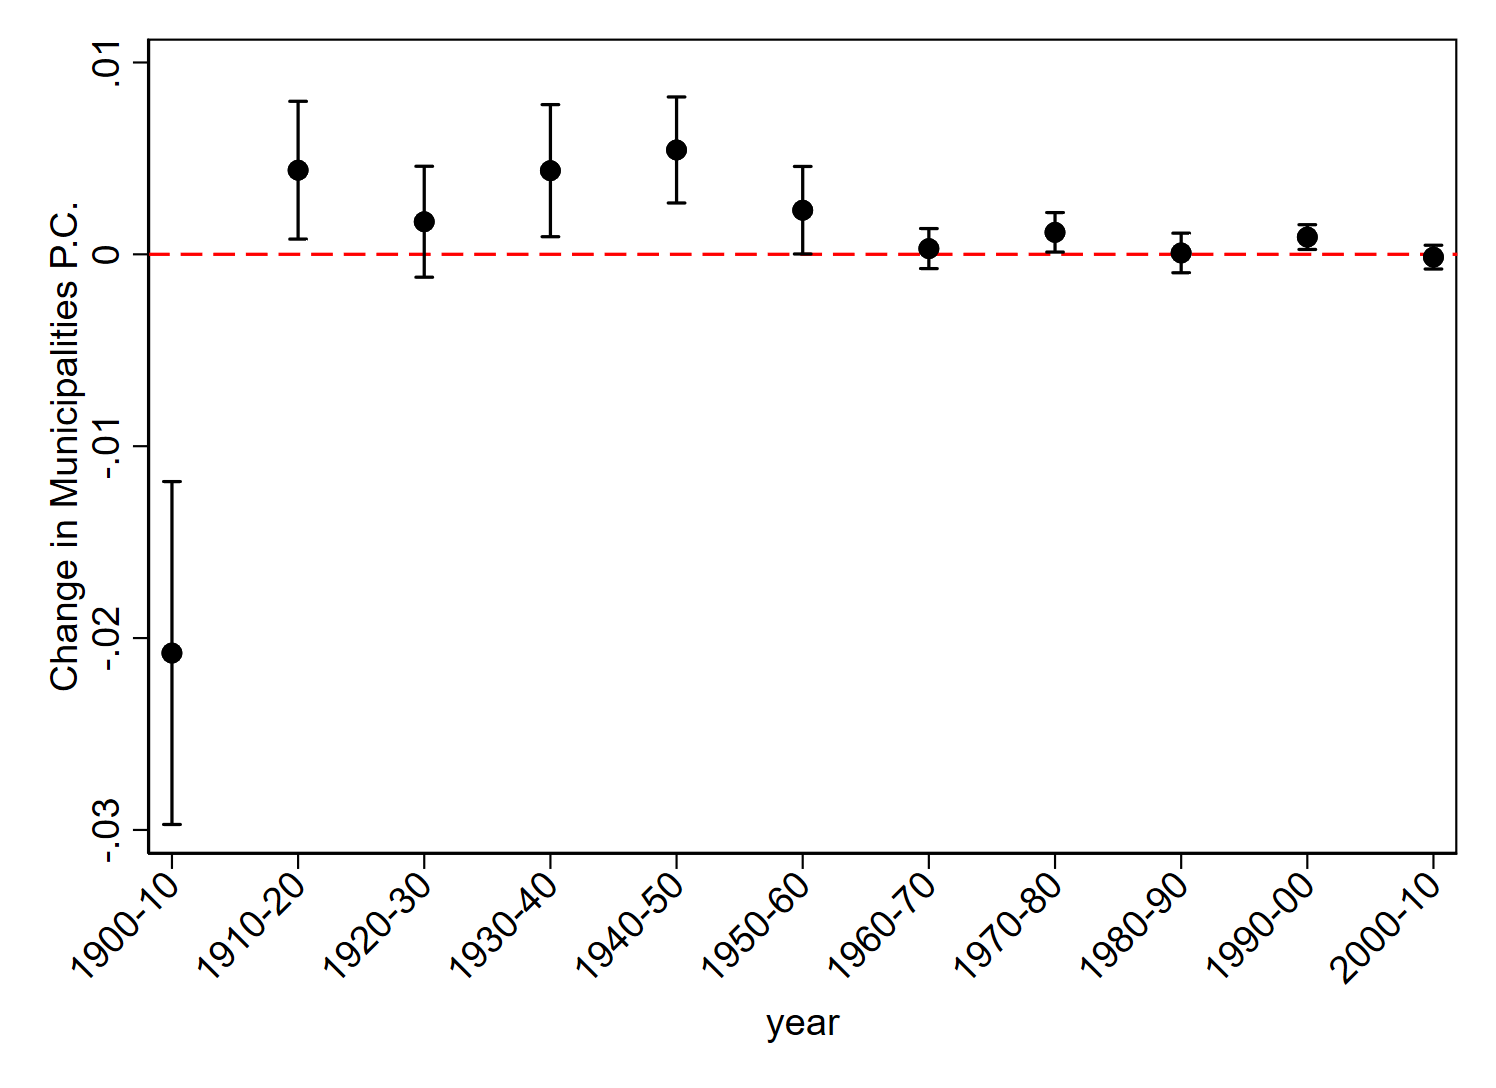
\includegraphics[width=0.7\linewidth]{figures/RR2/es_by_year.png}
	\caption{Repeated Cross Section, $\Delta$ munis P.C.}

\end{figure}
\clearpage

\begin{figure}
	\centering
	 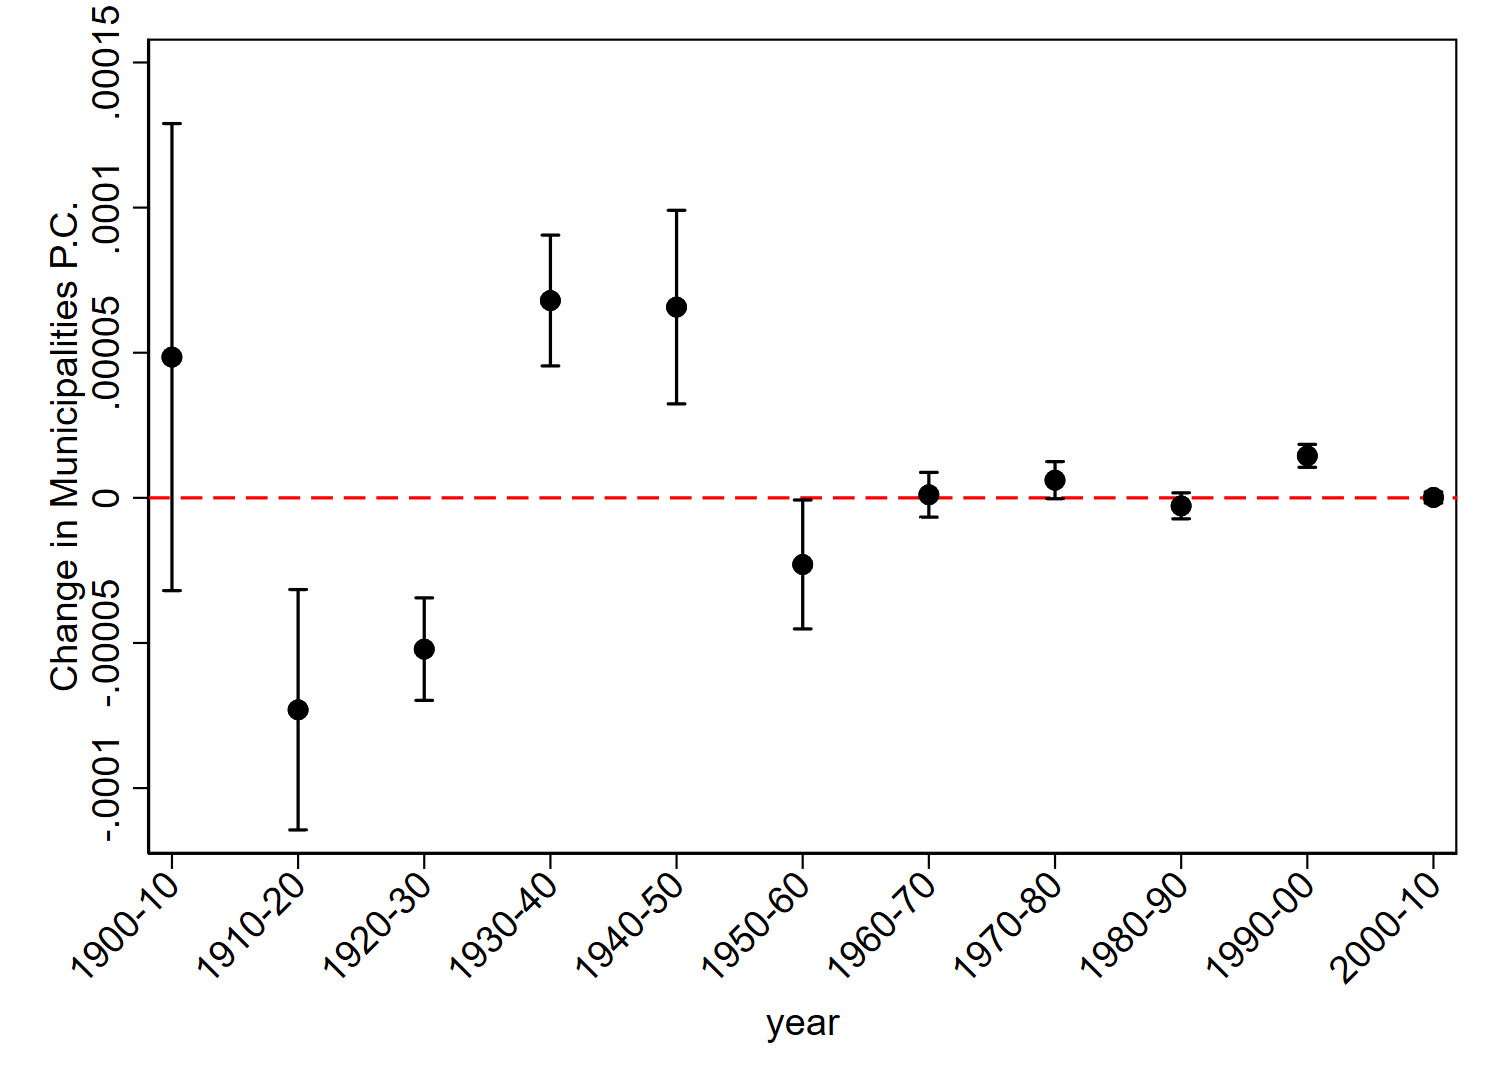
\includegraphics[width=0.7\linewidth]{figures/RR2/es_by_year_pct.png}
	\caption{Repeated Cross Section, $\frac{n_{70} - n_{40}}{Pop_{40}}$}
\end{figure}

\begin{figure}
	\centering
	 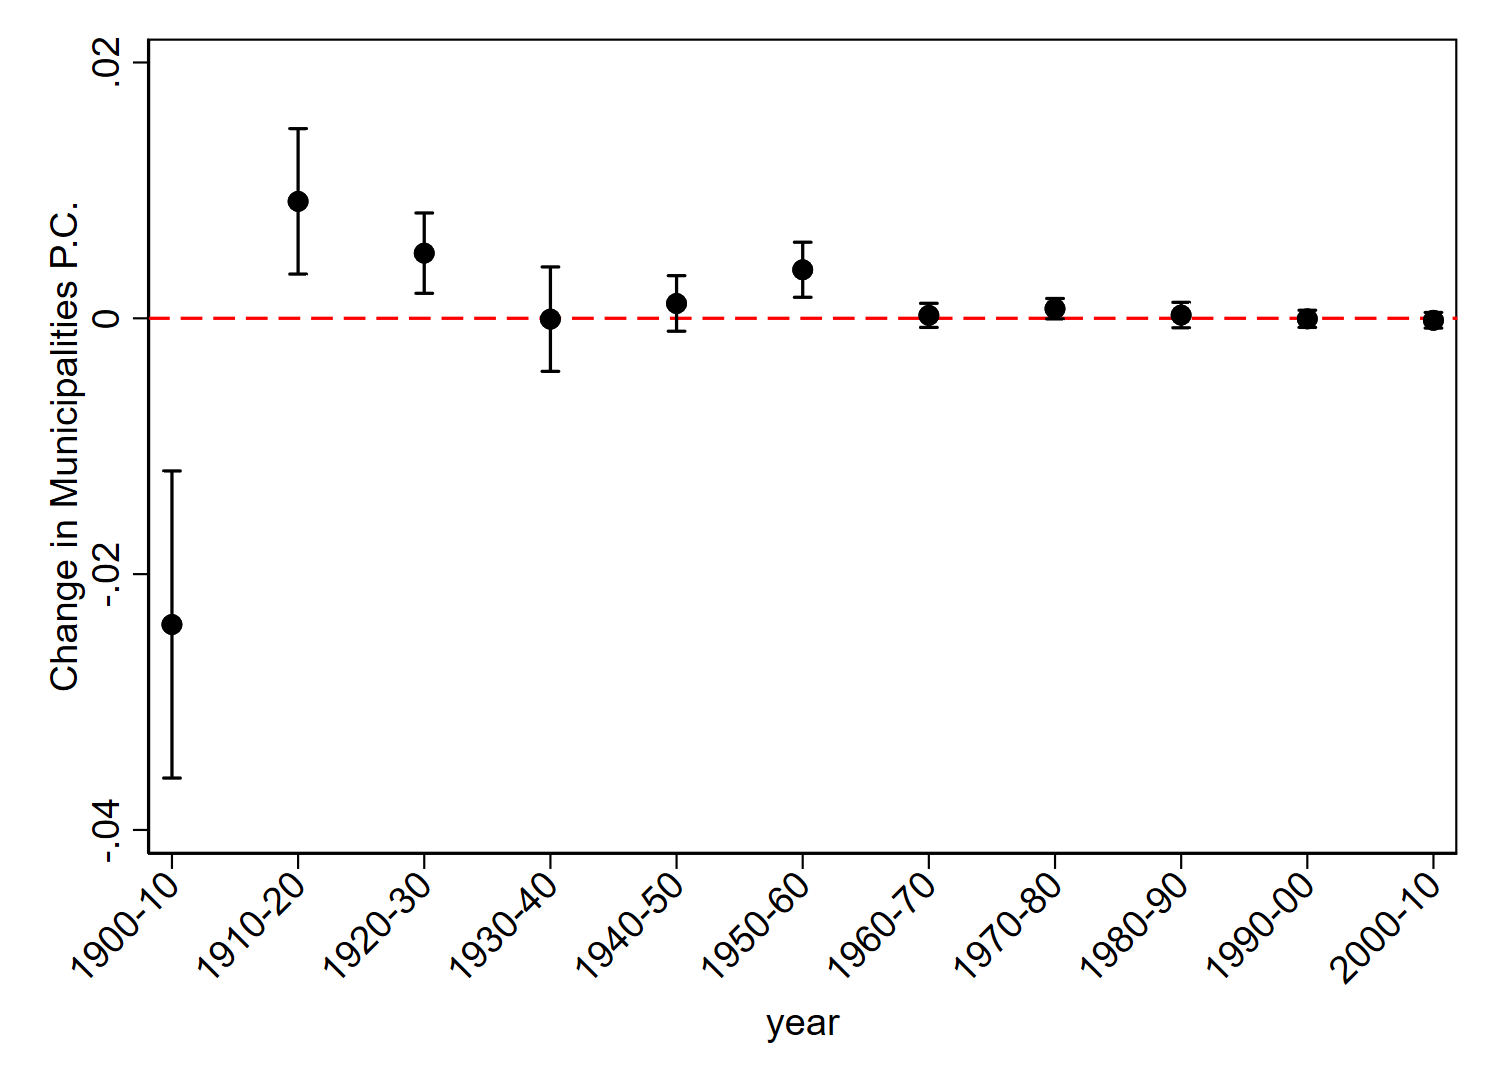
\includegraphics[width=0.7\linewidth]{figures/RR2/es_by_year_decomp.png}
	\caption{Repeated Cross Section, Population Dilution Term}
\end{figure}

\begin{figure}
	\centering
	 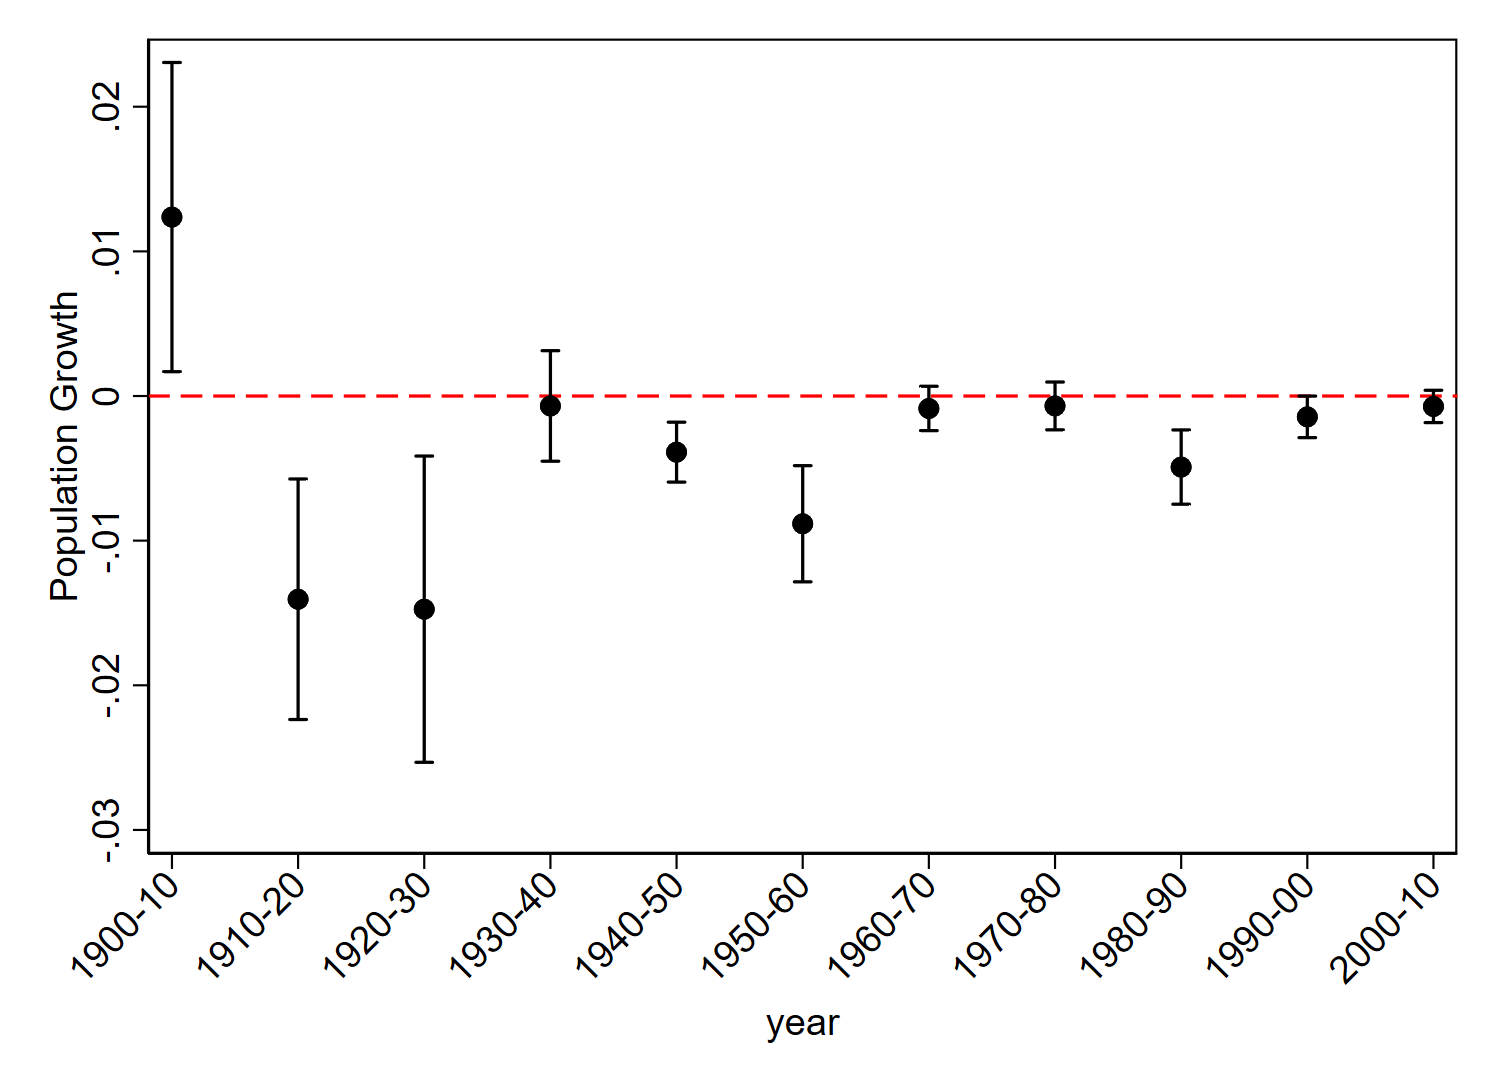
\includegraphics[width=0.7\linewidth]{figures/RR2/es_by_year_popgrowth.png}
	\caption{Repeated Cross Section, Population Growth}
\end{figure}
\clearpage
\section{Decadal 2SLS plots, Panel}
This table comes from creating a separate X and IV for each decade 1940-50, 1950-60, and 1960-1970, then performing the 2SLS regression as a stacked panel. 
\begin{align}
	y_{it} =  \beta GM_{it} + \mathbf{X}_i' \zeta_t + \delta_t + \epsilon_{it}
\end{align}

\clearpage
\begin{table}
\footnotesize
\centering
\caption{Panel IV}
\begin{threeparttable}
\footnotesize
\begin{tabularx}{\textwidth}{l*{5}{>{\centering\arraybackslash}X}} \toprule \setlength{\tabcolsep}{15pt}
&\multicolumn{1}{c}{C. Goodman}&\multicolumn{3}{c}{Census of Governments}&\multicolumn{1}{c}{Census}\\\cmidrule(lr){2-2}\cmidrule(lr){3-5}\cmidrule(lr){6-6}
&\multicolumn{2}{c}{Municipalities}&\multicolumn{1}{c}{School districts}&\multicolumn{1}{c}{Special Districts}&\multicolumn{1}{c}{Main City Share}\\\cmidrule(lr){2-3}\cmidrule(lr){4-4}\cmidrule(lr){5-5}\cmidrule(lr){6-6}
&\multicolumn{1}{c}{(1)}&\multicolumn{1}{c}{(2)}&\multicolumn{1}{c}{(3)}&\multicolumn{1}{c}{(4)}&\multicolumn{1}{c}{(5)}\\
\cmidrule(lr){1-6}
\multicolumn{5}{l}{Panel A: First Stage $\widehat{GM}_t$}\\
\cmidrule(lr){1-6}
$\widehat{GM}_t$  &    0.458 &    0.458 &    0.476 &    0.458 &    0.458 \\
                &  (0.306)  &  (0.306)  &  (0.302)  &  (0.306)  &  (0.306)  \\
\cmidrule(lr){1-6}
F-Stat &   2.24 &   2.24 &   2.49 &   2.24 &   2.24 \\
\cmidrule(lr){1-6}
\multicolumn{5}{l}{Panel B: IV 1940-70}\\
\cmidrule(lr){1-6}
 GM\_t &    0.026*** &    0.028*** &    0.677*** &    0.077** &    -2.543*** \\
                &  (0.010)  &  (0.010)  &  (0.233)  &  (0.035)  &  (0.678)  \\
\cmidrule(lr){1-6}
Observations    &      390   &      390   &      354   &      390   &      390   \\
\bottomrule \end{tabularx}

\end{threeparttable}
\end{table}
\clearpage


\section{Decadal 2SLS plots, Split}
These figures come from creating a separate X and IV for each decade 1940-50, 1950-60, and 1960-1970, then performing the 2SLS regression separately for each year.  
\begin{align}
	y_{it} =  \beta_t GM_{it} + \mathbf{X}_i' \zeta_t + \delta_t + \epsilon_{it}
\end{align}


\clearpage
\begin{figure}
	\centering
	 
\includegraphics[width=0.7\linewidth]{figures/RR2/cgoodman_split_IV.png}
	\caption{Decadal 2SLS, C.Goodman Munis}

\end{figure}


\clearpage
\begin{figure}
	\centering
	 
\includegraphics[width=0.7\linewidth]{figures/RR2/gen_muni_split_IV.png}
	\caption{Decadal 2SLS, CoG Munis}

\end{figure}


\clearpage
\begin{figure}
	\centering
	 
\includegraphics[width=0.7\linewidth]{figures/RR2/schdist_ind_split_IV.png}
	\caption{Decadal 2SLS, School Districts}

\end{figure}


\clearpage
\begin{figure}
	\centering
	 
\includegraphics[width=0.7\linewidth]{figures/RR2/spdist_split_IV.png}
	\caption{Decadal 2SLS, Special Districts}

\end{figure}

\clearpage
\begin{figure}
	\centering
	 
\includegraphics[width=0.7\linewidth]{figures/RR2/totfrac_split_IV.png}
	\caption{Decadal 2SLS, Main City Share}

\end{figure}
\clearpage



\end{document}
